\documentclass[compress,12pt]{beamer}%handout,compress,

\usepackage{fontspec}
  \setmainfont[Scale=1.1,Ligatures={Common},Numbers={Proportional}]{Doulos SIL}
  \setsansfont[Ligatures={Common},Numbers={Proportional}]{Proxima Nova} 
  \setmonofont[Scale=0.8]{Monaco} 
  \defaultfontfeatures{Mapping=tex-text} % converts LaTeX specials (``quotes'' --- dashes etc.) to unicode
  \newcommand{\ipa}[1]{\textrm{#1}}
  \newcommand{\ort}[1]{\textrm{⟨#1⟩}}
  \newcommand{\gli}[1]{`#1'}
  \newcommand{\pse}[1]{\textit{#1}}

\usepackage[american]{babel}
\usepackage{csquotes}
\usepackage[backend=biber,style=apa,uniquename=false,url=false,maxcitenames=2,isbn=false, doi=false, firstinits=false]{biblatex}
  \DeclareLanguageMapping{english}{english-apa}
  \addbibresource{MyRefs.bib}
  \AtBeginBibliography{\tiny}

\usepackage{booktabs,xcolor,colortbl,expex,tikz}
\usepackage{amsmath,amssymb}
  \newcommand{\Env}{/ \rule{2em}{.5pt}} %Defines the / _  (the `phonological environment' line) 
  
\usepackage[activate=pageopen,noplaybutton,transparent]{media9}

\newcommand\Wider[2][3em]{%
\makebox[\linewidth][c]{%
  \begin{minipage}{\dimexpr\textwidth+#1\relax}
  \raggedright#2
  \end{minipage}%
  }%
}

\DeclareTextFontCommand{\emph}{\color{pinkish}}

%\definecolor{greenish}{RGB}{76,153,0}
%\definecolor{orangish}{RGB}{255,75,51}
\definecolor{greenish}{HTML}{00A08A}
\definecolor{pinkish}{HTML}{FF0000}
\definecolor{yellowish}{HTML}{F2AD00}
\definecolor{orangish}{HTML}{F98400}
\definecolor{bluish}{HTML}{5BBCD6}

\useoutertheme[subsection=false]{miniframes}
\usetheme{default}
\usecolortheme{seagull}
\usefonttheme{professionalfonts}
\setbeamercolor{frametitle}{fg=yellowish, bg=white}
\setbeamercolor{title}{fg=white, bg=yellowish}
\setbeamercolor{block title}{bg=bluish,fg=black}
\setbeamerfont{block title}{size=\large}
\setbeamerfont{block body}{size=\normalsize}
\setbeamercovered{transparent}
\resetcountonoverlays{excnt}
\setbeamercolor{alerted text}{fg=pinkish}
\setbeamertemplate{itemize/enumerate body begin}{\normalsize}
\setbeamertemplate{itemize/enumerate subbody begin}{\small}

%\includeonlyframes{part1}

\title[DT: Boundary]{\Large Discourse Transcription: Transitional Continuity}
\author[Bradley McDonnell]{\normalsize Bradley McDonnell}
\institute{\normalsize\color{bluish}{LING710\\University of Hawai‘i at Mānoa}}

\begin{document}
  \begin{frame}[label=intro]
      \titlepage
  \end{frame}

\section{Introduction}
\subsection{Boundary intonation}  
  \begin{frame}{Boundary intonation}
    \begin{itemize}
      \item Intonation is meaningful to participants.
      \item \emph{For example,} speakers often use intonation to signal whether they intend to continue speaking, and listeners are attentive to these cues.
    \end{itemize}
  \end{frame}
  
  \begin{frame}{Boundary intonation in DT}
   \begin{itemize}
     \item DT can provide a useful representation of the more \textit{interactionally} critical intonational information.
     \item Crucially differs from ToBI and other more phonologically detailed systems that are interested in the (meaningful) acoustic realization of F0.
    \end{itemize}
  \end{frame}
  
\subsection{Translational continuity}
  \begin{frame}{Transitional continuity (function)}
    \begin{itemize}
      \item[] \emph{Transitional continuity:}
      \\
      marks \textit{the degree of continuity} which occurs at the transition point between IUs.
    \begin{itemize}
      \item When a speaker arrives at the end of an IU, poised to continue – or not continue – on to the next,\\the intonation contour usually gives a fairly clear indication of whether the discourse business at hand will be continued, or has finished.
      \begin{itemize}
        \item \ldots or is even occasioning a response.
      \end{itemize}
    \end{itemize}
    \end{itemize}
    \end{frame}
    
    \begin{frame}{Transitional continuity (function)}
       \begin{itemize}
         \item We focus on three general contours:
          \begin{enumerate}
            \item {\color{greenish}Final}
            \item {\color{greenish}Continuing}
            \item {\color{greenish}Appeal}
          \end{enumerate}
        \end{itemize}
    \end{frame}
    
    \begin{frame}{Transitional continuity (form)}
      \begin{itemize}
          \item While the intonation contour classes in this set are defined in terms of their function, each category will be more or less consistently realized by a specific form:
          \begin{itemize}
            \item a specific acoustic contour, or set of contours, where each member of the set is determined by its context.
          \end{itemize}
        \end{itemize}
    \end{frame}
    
    \begin{frame}{Transitional continuity (form)}
      \begin{itemize}
        \item Range of phonetic realizations for a given boundary intonation class differs from one language to the next:
          \begin{itemize}
            \item this is one reason for using functionally based categories.
            \item this helps to ensure that similar intonational functions will be written similarly across languages, \ldots
            \item facilitating comparison even where acoustic realizations differ.
          \end{itemize}
        \end{itemize}
    \end{frame}
    
  \begin{frame}{Transitional continuity}
    \begin{center}
      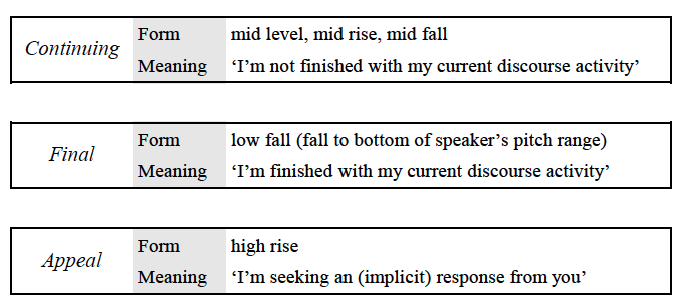
\includegraphics[width=0.9\textwidth]{images/IU_Continuities.png}
      \\
      \hfill {\color{bluish}\tiny Du Bois (in prep) \textit{Representing Discourse}}
    \end{center}
  \end{frame}
  \begin{frame}
    \begin{description}
      \item[\emph{NOTE:}] Punctuation in DT \textit{always} represents intonation classes. It is \textit{never} used to represent grammatical information. 
    \end{description}
  \end{frame}

\section{Examples}
\subsection{Final} 
  \begin{frame}{Final}
    \begin{itemize}
      \item[] \emph{Final intonation contour} = \textit{while it is being uttered, there is no indication that the speaker intends to continue speaking after the current IU.}
      \begin{itemize}
        \item This transitional continuity is marked by a \emph{period (.)}
        \item In English (and many other languages), final is marked by a fall to low pitch.
      \end{itemize}
    \end{itemize}  
  \end{frame}
  
  \begin{frame}{Final boundary intonation}
    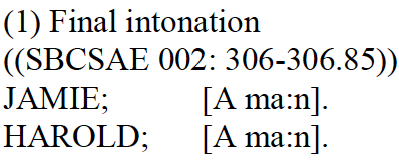
\includegraphics[width=0.5\textwidth]{images/Final_Ex1.png}\\
    \includemedia[
      label=Final_Ex1,
      addresource=audio/BoundarySample1.mp3,
      flashvars={
      source=audio/BoundarySample1.mp3
      }
      ]{\color{greenish}\fbox{\small play}}{APlayer.swf}
  \end{frame}

  \begin{frame}{Final boundary intonation}
    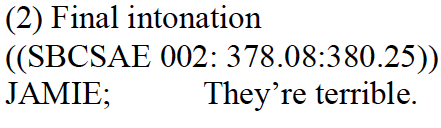
\includegraphics[width=0.5\textwidth]{images/Final_Ex2.png}\\
    \includemedia[
      label=Final_Ex2,
      addresource=audio/BoundarySample2.mp3,
      flashvars={
      source=audio/BoundarySample2.mp3
      }
      ]{\color{greenish}\fbox{\small play}}{APlayer.swf}
  \end{frame}  
  
  \begin{frame}{Final boundary intonation}
    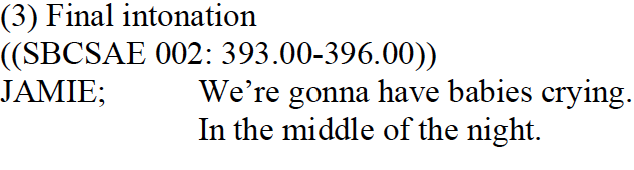
\includegraphics[width=0.75\textwidth]{images/Final_Ex3.png}\\
    \includemedia[
      label=Final_Ex3,
      addresource=audio/BoundarySample3.mp3,
      flashvars={
      source=audio/BoundarySample3.mp3
      }
      ]{\color{greenish}\fbox{\small play}}{APlayer.swf}
  \end{frame}

\subsection{Continuing} 

  \begin{frame}{Continuing}
    \begin{itemize}
      \item[] \emph{Continuing intonation contour} = \textit{while it is being uttered, the speaker intends to continue speaking after the current IU.}
      \begin{itemize}
        \item This transitional continuity is marked by a \emph{comma (,)}
        \item In English (and other languages), fall to mid-level pitch, \ldots
        \item but it may have other realizations as well, each of which presumably has slightly different pragmatic implications
        \begin{itemize} 
          \item  for example, a terminal pitch that remains level, 
          \item a very slight rise in pitch at the end of the IU, 
          \item a pitch that falls slightly but not low enough to be considered final.
      \end{itemize}
      \item In practice the comma represents a broad cover symbol for a variety of non-final contours\ldots
    \end{itemize}
    \end{itemize}  
  \end{frame}

  \begin{frame}{Continuing boundary intonation}
    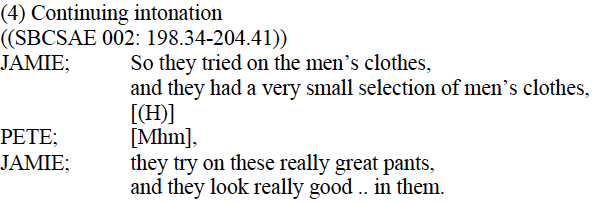
\includegraphics[width=0.85\textwidth]{images/Cont_Ex4.png}\\
    \includemedia[
      label=Cont_Ex4,
      addresource=audio/BoundarySample4.mp3,
      flashvars={
      source=audio/BoundarySample4.mp3
      }
      ]{\color{greenish}\fbox{\small play}}{APlayer.swf}
  \end{frame}

  \begin{frame}{Continuing boundary intonation}
    \begin{columns}[T]
    \begin{column}{0.4\textwidth}
    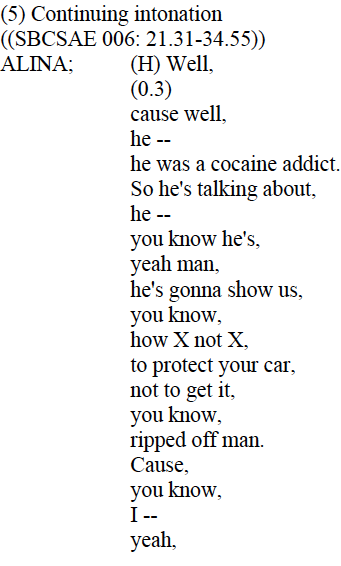
\includegraphics[width=1\textwidth]{images/Cont_Ex5.png}
    \end{column}
    \begin{column}{0.5\textwidth}
    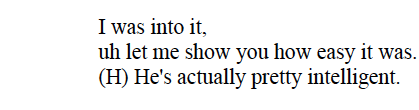
\includegraphics[width=1\textwidth]{images/Cont_Ex5b.png}\\
    \hfill\includemedia[
      label=Cont_Ex5,
      addresource=audio/BoundarySample5.mp3,
      flashvars={
      source=audio/BoundarySample5.mp3
      }
      ]{\color{greenish}\fbox{\small play}}{APlayer.swf}
    \end{column}
    \end{columns}
  \end{frame}  
  
\subsection{Appeal}

  \begin{frame}{Appeal}
    \begin{itemize}
      \item[] \emph{Appeal intonation contour} = \textit{when a speaker, in producing an utterance, overtly seeks a validating response from a listener.}
      \begin{itemize}
        \item This transitional continuity is marked by a \emph{question mark (?)}
        \item In English (and many other languages), appeal is realized by a marked high rise in pitch at the end of the IU.
        \begin{itemize} 
          \item most commonly a yes-no question, but not all yes-no questions are said with the appeal contour, 
          \item in such cases the question should not be written with a question mark.
        \end{itemize}
      \end{itemize}
    \end{itemize}  
  \end{frame}

  \begin{frame}{Appeal boundary intonation}
    \begin{itemize}
        \item appeal contour may be used in contexts other than a yes-no question,  
        \item in such cases the question mark should be used.
        \item[] (speaker nods in agreement with example below)    
    \end{itemize}
    \hfill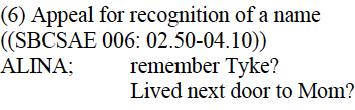
\includegraphics[width=0.6\textwidth]{images/Appeal_Ex6.png}\\
    \hfill\includemedia[
      label=Appeal_Ex6,
      addresource=audio/BoundarySample6.mp3,
      flashvars={
      source=audio/BoundarySample6.mp3
      }
      ]{\color{greenish}\fbox{\small play}}{APlayer.swf}
  \end{frame}

  \begin{frame}{Appeal boundary intonation}
    \begin{itemize}
        \item question mark can be followed by a period or a comma 
        \item indicating whether the IU with the appeal contour is considered to be final or continuing, respectively.  
    \end{itemize}  
    \hfill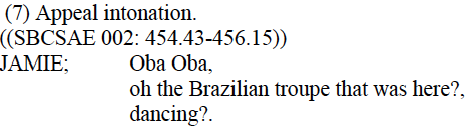
\includegraphics[width=0.75\textwidth]{images/Appeal_Ex7.png}\\
    \hfill\includemedia[
      label=Appeal_Ex7,
      addresource=audio/BoundarySample7.mp3,
      flashvars={
      source=audio/BoundarySample7.mp3
      }
      ]{\color{greenish}\fbox{\small play}}{APlayer.swf}
  \end{frame}

  \begin{frame}{Appeal boundary intonation}
    \begin{itemize}
        \item question mark can be followed by a period or a comma 
        \item indicating whether the IU with the appeal contour is considered to be final or continuing, respectively.  
    \end{itemize}  
    \hfill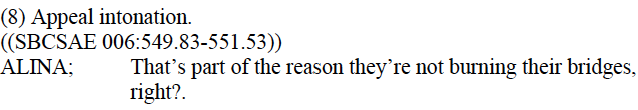
\includegraphics[width=1\textwidth]{images/Appeal_Ex8.png}\\
    \hfill\includemedia[
      label=Appeal_Ex8,
      addresource=audio/BoundarySample8.mp3,
      flashvars={
      source=audio/BoundarySample8.mp3
      }
      ]{\color{greenish}\fbox{\small play}}{APlayer.swf}
  \end{frame}
  
  \begin{frame}{Appeal boundary intonation}
    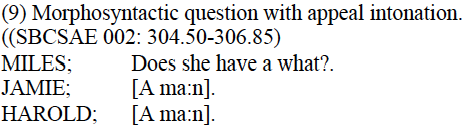
\includegraphics[width=0.8\textwidth]{images/Appeal_Ex9.png}\\
    \includemedia[
      label=Appeal_Ex9,
      addresource=audio/BoundarySample9.mp3,
      flashvars={
      source=audio/BoundarySample9.mp3
      }
      ]{\color{greenish}\fbox{\small play}}{APlayer.swf}
  \end{frame}
  
  \begin{frame}{Appeal boundary intonation}
    \begin{itemize}
      \item the question mark is \textit{not} used for a grammatical question uttered with intonations other than the appeal contour,
      \item such as declarative contours.
    \end{itemize}
    \hfill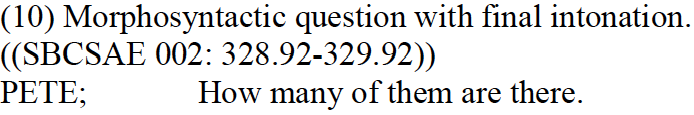
\includegraphics[width=0.8\textwidth]{images/Appeal_Ex10.png}\\
    \hfill\includemedia[
      label=Appeal_Ex10,
      addresource=audio/BoundarySample10.mp3,
      flashvars={
      source=audio/BoundarySample10.mp3
      }
      ]{\color{greenish}\fbox{\small play}}{APlayer.swf}
  \end{frame}
   
  
\section{Conclusion}
\subsection{Choosing the right symbol}
  \begin{frame}{Choosing a boundary symbol}
    \begin{center}
      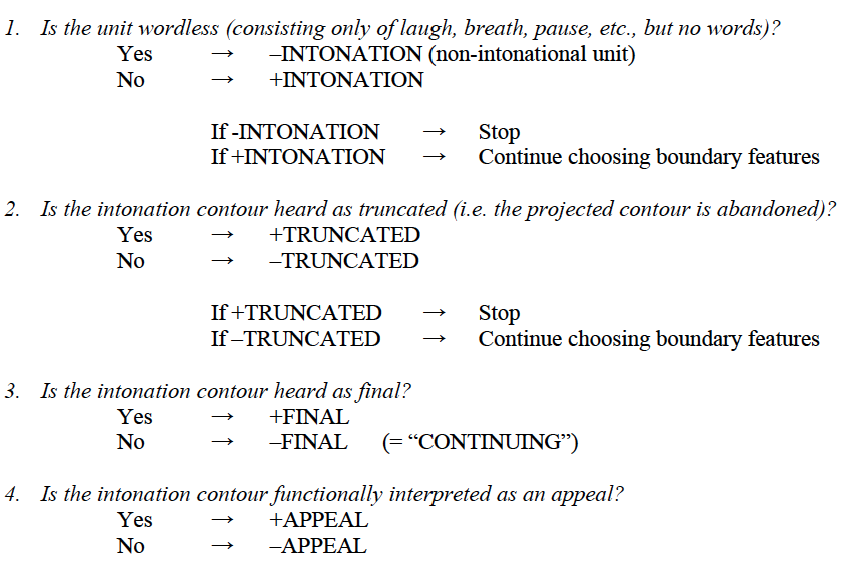
\includegraphics[width=0.9\textwidth]{images/IU_Questions.png}
      \\
      \hfill {\color{bluish}\tiny Du Bois (in prep) \textit{Representing Discourse}}
    \end{center}
  \end{frame}
  
  \subsection{Practice}
  \begin{frame}{Let's practice\ldots}
  \begin{center}
      \includemedia[
      label=Practice,
      addresource=audio/SBC005_0172-0212.mp3,
      flashvars={
      source=audio/SBC005_0172-0212.mp3
      }
      ]{\color{greenish}\fbox{\hspace{2cm}\Large play\hspace{2cm}}}{APlayer.swf}
      \end{center}
  \end{frame}
\end{document}